\documentclass{article}
\usepackage{parskip}
\usepackage{amsmath}
\usepackage[dvipdfmx]{graphicx}
\usepackage{cleveref}

\newcommand{\myparagraph}[1]{\paragraph{#1}\mbox{}\\}

\begin{document}

ある長方形を3つの長方形に分割する方法は,
ある1辺に平行な2本の線分によって分割する方法(\cref{type-i})か,
各辺にそれぞれ平行な1本ずつの線分によって分割する方法(\cref{type-t})のいずれかのみである。
これらをそれぞれI型,T型と呼ぶことにする。

\begin{figure}[h]
    \begin{center}
        \begin{tabular}{c}
            \begin{minipage}{0.33\hsize}
                \begin{center}
                    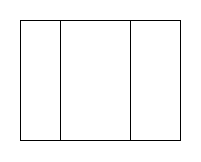
\includegraphics[width=100pt]{type-i.png}
                    \caption{I型}
                    \label{type-i}
                \end{center}
            \end{minipage}

            \begin{minipage}{0.33\hsize}
                \begin{center}
                    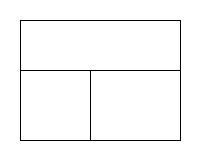
\includegraphics[width=100pt]{type-t.png}
                    \caption{T型}
                    \label{type-t}
                \end{center}
            \end{minipage}
        \end{tabular}
    \end{center}
\end{figure}

$\Delta S = S_{max} - S_{min}$とおく。
$H, W$の少なくとも一方が3で割り切れるならば,
I型の分割によってちょうど3等分することができ,
このとき$\Delta S = 0$である。
以下,$H, W$のいずれも3で割り切れないときを考える。

\myparagraph{[1] I型に分割するとき}

まず,(\cref{type-i})のように縦の辺に平行な2本の線分を引いて分割する場合を考える。
$W = 2$のときはI型の分割が存在しないから,
2以上の整数$k$を用いて$W = 3k + 1$または$W = 3k - 1$と表せるときを考えればよい。

このとき,$\Delta S$が最小となるような
3つの長方形の幅の組は$k, k, k + 1$または$k, k, k - 1$であり,
このように分割すれば$\Delta S = H$ である。

同様に,横の辺に平行な2本の線分を引いて分割する場合も考えると,
I型の分割をするときの$\Delta S$の最小値は
\begin{equation}
    \label{min-i}
    \min \{H, W\}
\end{equation}
である。

\myparagraph{[2] T型に分割するとき}

まず,(\cref{type-t})のように1辺の長さが$W$の長方形ができるように分割する場合を考える。
T型の分割は任意の$W, H$に対して存在する。

(\cref{type-t})下部の2つの長方形の幅の差が最小となるような
2つの長方形の幅の組は
\begin{equation}
    \label{w2}
    \left\lfloor \dfrac{W}{2} \right\rfloor,\ \left\lceil \dfrac{W}{2} \right\rceil
\end{equation}
である。これら2つの長方形の高さを$h$とおくと,3つの長方形の面積はそれぞれ,
\begin{eqnarray*}
    &A(h) = W (H - h), \\
    &B(h) = h \left\lfloor \dfrac{W}{2} \right\rfloor \\
    &C(h) = h \left\lceil  \dfrac{W}{2} \right\rceil
\end{eqnarray*}
であり,$A(h)$は$h$に関して単調増加,$B(h), C(h)$は$h$に関して単調減少で
\begin{equation}
    \label{b_c}
    B(h) \leq C(h)
\end{equation}
が成り立つ。

\myparagraph{[2-1] $W$が偶数のとき}

$W$が偶数ならば,(\ref{w2})の2数は互いに等しいので,
\begin{equation*}
    B(l) = C(l) = \dfrac{W}{2} h
\end{equation*}
である。

$A(h), B(h), C(h)$の単調性と,
\begin{equation*}
    A(l) > B(l)
    \Longleftrightarrow
    \frac{2}{3} H > h
\end{equation*}
すなわち $h = \dfrac{2}{3} H$ を境に$A(h)$と$B(h)$の
大小関係が逆転することに注意すれば,$\Delta S$が最小となるのは,$h$の値が
\begin{equation*}
    h_1 = \left\lfloor \frac{2}{3} H \right\rfloor
    \hspace{15pt} \mbox{または} \hspace{15pt}
    h_2 = \left\lceil  \frac{2}{3} H \right\rceil
\end{equation*}
のときであり,このとき,$\Delta S$の最小値は
\begin{equation}
    \label{min-t1}
    \begin{cases}
        \vspace{15pt}
        A(h) - B(h) & (h = h_1 \mbox{のとき}) \\
        B(h) - A(h) & (h = h_2 \mbox{のとき})
    \end{cases}
\end{equation}
である。これらの値は$W, H$のみに依存する。

\myparagraph{[2-2] $W$が奇数のとき}

(\ref{b_c})により,$A(h), B(h), C(h)$の大小関係は次の3通りである:
\begin{eqnarray}
    \label{abc1}
    B(h) \leq A(h) \leq C(h) \\
    \label{abc2}
    A(h) \leq B(h) \leq C(h) \\
    \label{abc3}
    B(h) \leq C(h) \leq A(h)
\end{eqnarray}

ここで,
\begin{equation*}
    B(h) \leq A(h)
    \Longleftrightarrow
    h \leq
    \dfrac{WH}{ W + \left\lfloor \dfrac{W}{2} \right\rfloor }
\end{equation*}
\begin{equation*}
    A(h) \leq C(h)
    \Longleftrightarrow
    \dfrac{WH}{ W + \left\lceil \dfrac{W}{2} \right\rceil }
    \leq h
\end{equation*}
であることから,(\ref{abc1})を満たす$h$は存在しない。

$A(h), B(h), C(h)$の単調性と,
\begin{equation*}
    h = \dfrac{WH}{ W + \left\lfloor \dfrac{W}{2} \right\rfloor }
    \hspace{15pt} \mbox{および} \hspace{15pt}
    h = \dfrac{WH}{ W + \left\lceil  \dfrac{W}{2} \right\rceil }
\end{equation*}
を境に$A(h)$と$B(h)$,$A(h)$と$C(h)$の大小関係がそれぞれ逆転することに注意すれば,
$\Delta S$が最小となるのは,$h$の値が
\begin{equation*}
    h_3 =
    \left\lceil
        \dfrac{WH}{ W + \left\lfloor \dfrac{W}{2} \right\rfloor }
    \right\rceil
    \hspace{15pt} \mbox{または} \hspace{15pt}
    h_4 =
    \left\lfloor
        \dfrac{WH}{ W + \left\lceil  \dfrac{W}{2} \right\rceil }
    \right\rfloor
\end{equation*}
のときであり,このとき,$\Delta S$の最小値は
\begin{equation}
    \label{min-t2}
    \begin{cases}
        \vspace{15pt}
        A(h) - B(h) & (h = h_3 \mbox{のとき}) \\
        B(h) - A(h) & (h = h_4 \mbox{のとき})
    \end{cases}
\end{equation}
である。これらの値は$W, H$のみに依存する。

以上より,求める最小値は(\ref{min-i}), (\ref{min-t1}), (\ref{min-t2})のうち最小のものである。

\end{document}
